%\documentclass[first=dgreen,second=purple,logo=yellowexc]{aaltoslides}
\documentclass{beamer}
%\documentclass{aaltoslides} % DEFAULT
%\documentclass[first=purple,second=lgreen,logo=redque,normaltitle,nofoot]{aaltoslides} % SOME OPTION EXAMPLES

\usepackage[latin9]{inputenc}
\usepackage[T1]{fontenc}
\usepackage{graphicx}
\usepackage{amssymb,amsmath}
\usepackage{url}
\usepackage{lastpage}
\setbeamercovered{transparent}

\usepackage[SCI]{aaltologo}


\usepackage{scrextend}
\changefontsizes{10pt}


\newcommand{\bmx}[0]{\begin{bmatrix}}
\newcommand{\emx}[0]{\end{bmatrix}}
\newcommand{\qt}[1]{\left<#1\right>}
\newcommand{\qexp}[1]{\left<#1\right>}
\newcommand{\qlay}[1]{\left[#1\right]}
\newcommand{\vect}[1]{\mathbf{#1}}
\newcommand{\vects}[1]{\boldsymbol{#1}}
\newcommand{\matr}[1]{\mathbf{#1}}
\newcommand{\var}[0]{\operatorname{Var}}
\newcommand{\cov}[0]{\operatorname{Cov}}
\newcommand{\diag}[0]{\operatorname{diag}}
\newcommand{\matrs}[1]{\boldsymbol{#1}}
\newcommand{\va}[0]{\vect{a}}
\newcommand{\vb}[0]{\vect{b}}
\newcommand{\vc}[0]{\vect{c}}
\newcommand{\vh}[0]{\vect{h}}
\newcommand{\vv}[0]{\vect{v}}
\newcommand{\vf}[0]{\vect{f}}
\newcommand{\vx}[0]{\vect{x}}
\newcommand{\vy}[0]{\vect{y}}
\newcommand{\vg}[0]{\vect{g}}
\newcommand{\vr}[0]{\vect{r}}
\newcommand{\vq}[0]{\vect{q}}
\newcommand{\vm}[0]{\vect{m}}
\newcommand{\vs}[0]{\vect{s}}
\newcommand{\vw}[0]{\vect{w}}
\newcommand{\vL}[0]{\vect{L}}
\newcommand{\vp}[0]{\vect{p}}
\newcommand{\vz}[0]{\vect{z}}
\newcommand{\mW}[0]{\matr{W}}
\newcommand{\mG}[0]{\matr{G}}
\newcommand{\mX}[0]{\matr{X}}
\newcommand{\mY}[0]{\matr{Y}}
\newcommand{\mK}[0]{\matr{K}}
\newcommand{\mH}[0]{\matr{H}}
\newcommand{\mQ}[0]{\matr{Q}}
\newcommand{\mU}[0]{\matr{U}}
\newcommand{\mR}[0]{\matr{R}}
\newcommand{\mV}[0]{\matr{V}}
\newcommand{\mA}{\matr{A}}
\newcommand{\mD}{\matr{D}}
\newcommand{\mC}{\matr{C}}
\newcommand{\mS}{\matr{S}}
\newcommand{\mI}{\matr{I}}
\newcommand{\mL}{\matr{L}}
\newcommand{\mzero}[0]{\matr{0}}
\newcommand{\td}[0]{\text{d}}
\newcommand{\valpha}[0]{\vects{\alpha}}
\newcommand{\vbeta}[0]{\vects{\beta}}
\newcommand{\vsig}[0]{\vects{\sigma}}
\newcommand{\vmu}[0]{\vects{\mu}}
\newcommand{\vone}[0]{\vects{1}}
\newcommand{\vzero}[0]{\vects{0}}
%\newcommand{\tf}[0]{\text{f}}
\newcommand{\tf}[0]{\text{m}}
\newcommand{\tdf}[0]{\text{dm}}
\newcommand{\TT}[0]{{\vects{\theta}}}
\newcommand{\grad}[0]{\nabla}
\newcommand{\N}[0]{\mathcal{N}}
\newcommand{\CC}[0]{\mathcal{C}}
\newcommand{\QQ}[0]{\mathbb{Q}}
\newcommand{\PP}[0]{\mathbb{P}}
\newcommand{\RR}[0]{\mathbb{R}}
\newcommand{\NN}[0]{\mathcal{N}}
\newcommand{\MM}[0]{\mathcal{M}}
\newcommand{\LL}[0]{\mathcal{L}}
\newcommand{\HH}[0]{\mathcal{H}}
\newcommand{\T}[0]{\mathcal{T}}
\newcommand{\BB}[0]{\mathcal{B}}
\newcommand{\KL}[0]{\text{KL}}
\newcommand{\CD}[0]{\text{CD}}
\newcommand{\sigmoid}{\sigma}
\newcommand{\E}[0]{\mathbb{E}}
\newcommand{\enabla}[0]{\ensuremath{%
    \overset{\raisebox{-0.3ex}[0.5ex][0ex]{%
    \ensuremath{\scriptscriptstyle e}}}{\nabla}}}
\newcommand{\enhnabla}[0]{\nabla_{\hspace{-0.5mm}e}\,}
\newcommand{\tred}[1]{\textcolor{red}{#1}}
\newcommand{\tblue}[1]{\textcolor{blue}{#1}}
\newcommand{\dd}[1]{\text{d}{#1}}

\DeclareMathOperator*{\argmin}{arg\,min}
\DeclareMathOperator*{\argmax}{arg\,max}

\newcommand{\dbm}{DBM}
\newcommand{\dbmptrbm}{DBM$^\text{DBN}_\text{RBM}$}
\newcommand{\dbmptdae}{DBM$^\text{sDAE}_\text{RBM}$}
\newcommand{\dbmptruslan}{DBM$^\text{S\&H}$}
\newcommand{\dbmptruslanrbm}{DBM$^\text{S\&H}_\text{RBM}$}
\newcommand{\dbmptruslanfvbm}{DBM$^\text{S\&H}_\text{FVBM}$}

\title{Deep Learning}

\author[K. Cho]{Kyunghyun Cho}
\institute[ICS]{Department of Information and Computer Science\\
Aalto University, School of Science\\kyunghyun.cho@aalto.fi}

%\aaltofootertext{Foundations and Advances in Deep Learning}{\today}{\arabic{page}/\pageref{LastPage}\ }

\date{21 March 2014}

\begin{document}

%%%%%%%%%%%%%%%%%%%%%%%%%%%%%%%%%%%%%%%%%%%%%%%%%%%%%%%%%%%%%%%%%%%%%%%%%%%%%%%%%%%%%%%%%%%%%

\frame{\titlepage}
%\aaltotitleframe

%%%%%%%%%%%%%%%%%%%%%%%%%%%%%%%%%%%%%%%%%%%%%%%%%%%%%%%%%%%%%%%%%%%%%%%%%%%%%%%%%%%%%%%%%%%%%

%\begin{frame}
%    \raggedright
%    This work was done under the supervision of Prof. Juha
%    Karhunen, Prof. Tapani Raiko and Dr. Alexander Ilin at
%    the Deep Learning and Bayesian Modeling Group,
%    Department of Information and Computer Science, Aalto
%    University School of Science between mid 2009 and early 2014.
%
%    \vspace{10mm}
%    \raggedleft
%    \AaltoLogoSmall{0.5}{!}{aaltoRed}
%
%\end{frame}

%\begin{frame}
%    \tableofcontents[ 
%    currentsubsection, 
%    %hideothersubsections, 
%    sectionstyle=show, 
%    subsectionstyle=show,
%    ] 
%\end{frame}

\section{Machine Learning \& Perception}

\begin{frame}{Machine Learning}
    \centering
    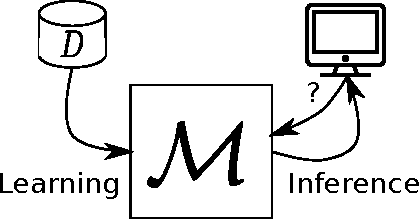
\includegraphics[width=0.55\textwidth]{machinelearning.pdf}

    \vspace{4mm}
    \raggedright
    \begin{enumerate}
        \item Let the model $\MM$ \tred{\textit{learn}} the data $D$
        \item Let the model $\MM$ \tblue{\textit{infer}} unknown
            quantities
    \end{enumerate}
\end{frame}

\begin{frame}{Machine Learning \& Perception}
    \vfill

    \centering
    \begin{minipage}{0.33\textwidth}
        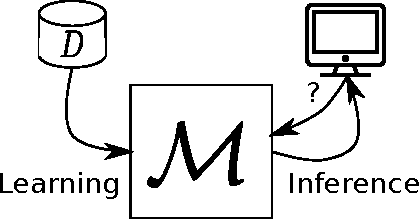
\includegraphics[width=\columnwidth]{machinelearning.pdf}
    \end{minipage}
    \hfill
    \begin{minipage}{0.65\textwidth}
        \raggedright
        \emph{Perception} is the organization, identification, and
        interpretation of \emph{sensory information} in order to
        represent and \emph{understand the environment}.
        
        \raggedleft
        {\scriptsize --Wikipedia}
    \end{minipage}

    \vspace{10mm}
    \begin{minipage}{0.44\textwidth}
        \centering
        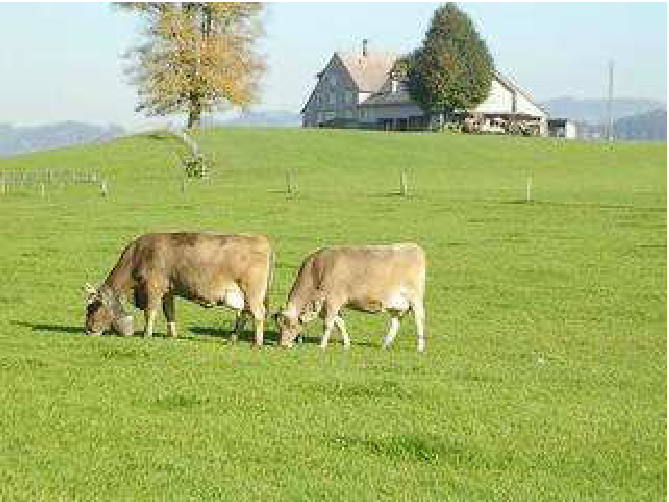
\includegraphics[width=0.8\columnwidth]{farabet_pami_img1.pdf}
    \end{minipage}
    \hfill
    $\to$
    \hfill
    \begin{minipage}{0.44\textwidth}
        \centering
        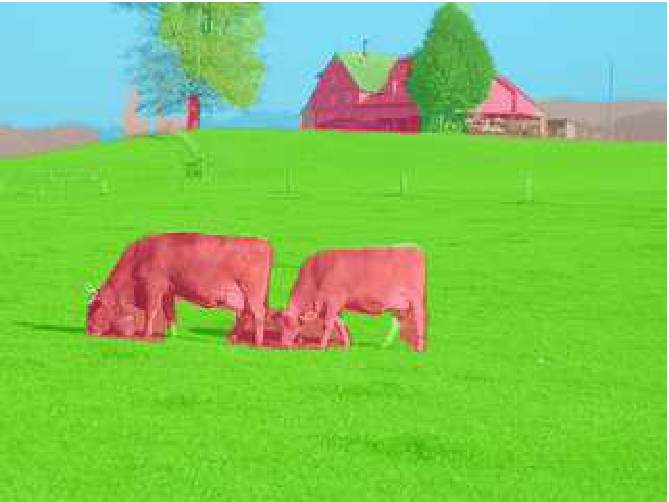
\includegraphics[width=0.8\columnwidth]{farabet_pami_img2.pdf}
    \end{minipage}
    \centering
    \vspace{1mm}
    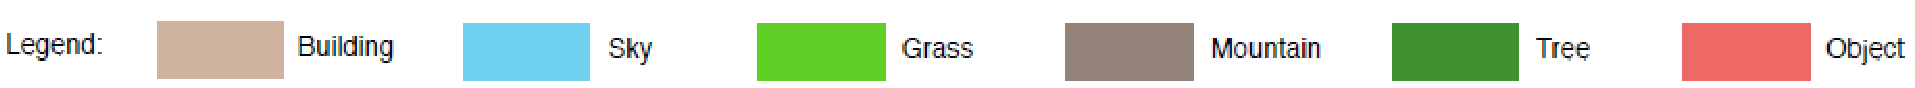
\includegraphics[width=0.8\textwidth]{farabet_pami_img_legend.pdf}
    \vspace{-3mm}
    \begin{flushright}
        \scriptsize (Farabet et al., 2013)
    \end{flushright}

    \vfill
\end{frame}

\begin{frame}{Machine Learning \& Perception: Examples}
    \centering
    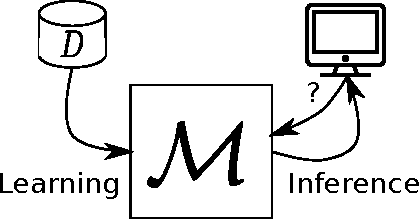
\includegraphics[width=0.55\textwidth]{machinelearning.pdf}

    \vspace{2mm}
    \begin{center}
    { \small
    \begin{tabular}{l | l | l}
        \bf Data & \bf Sensory Information & \bf Query\\
        \hline
        \hline
        Labeled Images &
        An image &
        Is a cat in the image? \\
        Transcribed Speech &
        A speech segment &
        What is this person saying?  \\
        Paraphrases &
        A pair of sentences &
        Is this sentence a paraphrase? \\
        Movie Ratings & 
        Ratings of $Y$ and by $X$ & 
        Will a user $X$ like a movie $Y$? \\
        Parallel Corpora &
        A Finnish sentence &
        What is ``moi'' in English?  
    \end{tabular}
    }
\end{center}
\end{frame}

\section{Deep Learning: Born Again}

\begin{frame}
    \centering

    A human possesses \emph{the} best machinery for perception,
    called a \emph{\bf brain}.

    \vspace{2em}
    But, how does our brain do it?

\end{frame}

\begin{frame}{Deep Learning: Motivated from Human Learning}

    \vfill

     \centering
     \begin{minipage}{0.32\textwidth}
         \centering
         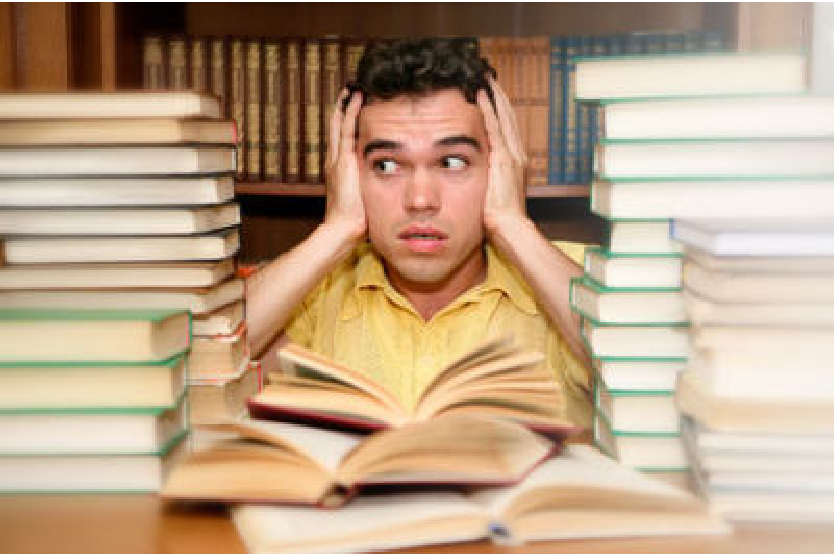
\includegraphics[width=0.9\columnwidth]{studying.pdf}
     \end{minipage}
     \hfill
     \begin{minipage}{0.32\textwidth}
         \centering
         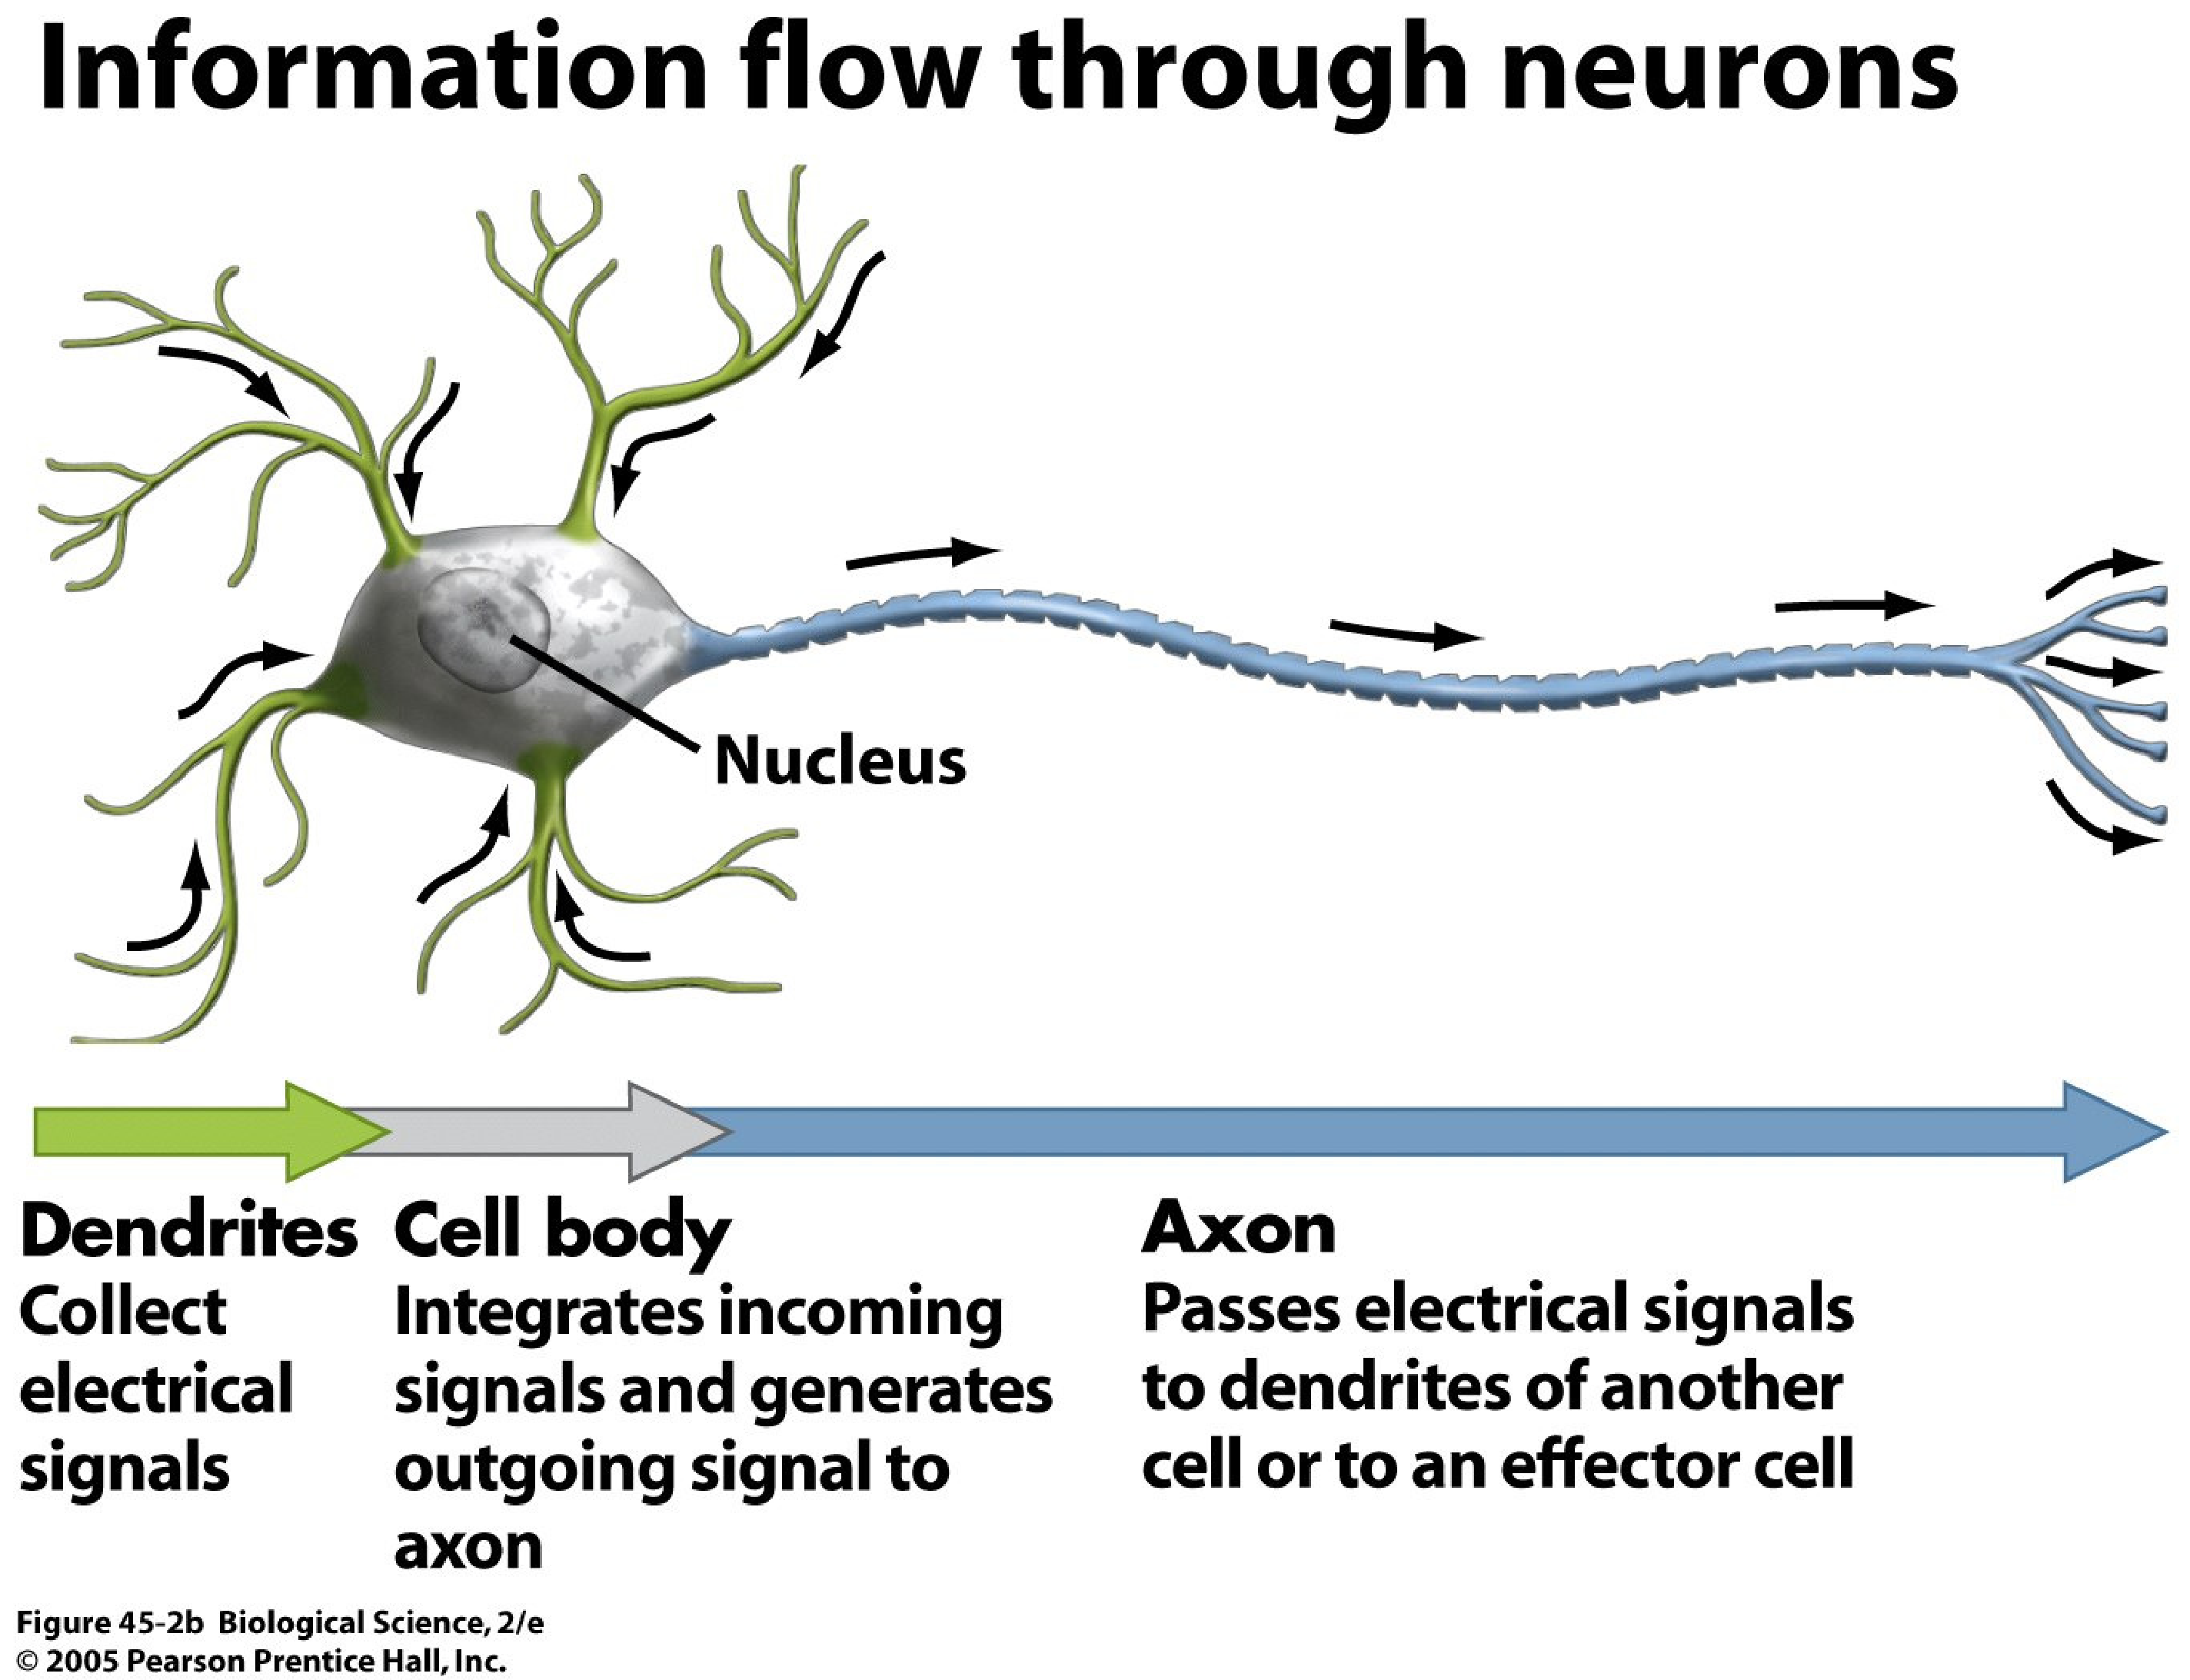
\includegraphics[width=0.9\columnwidth]{neuron.pdf}
     \end{minipage}
     \hfill
     \begin{minipage}{0.32\textwidth}
         \centering
         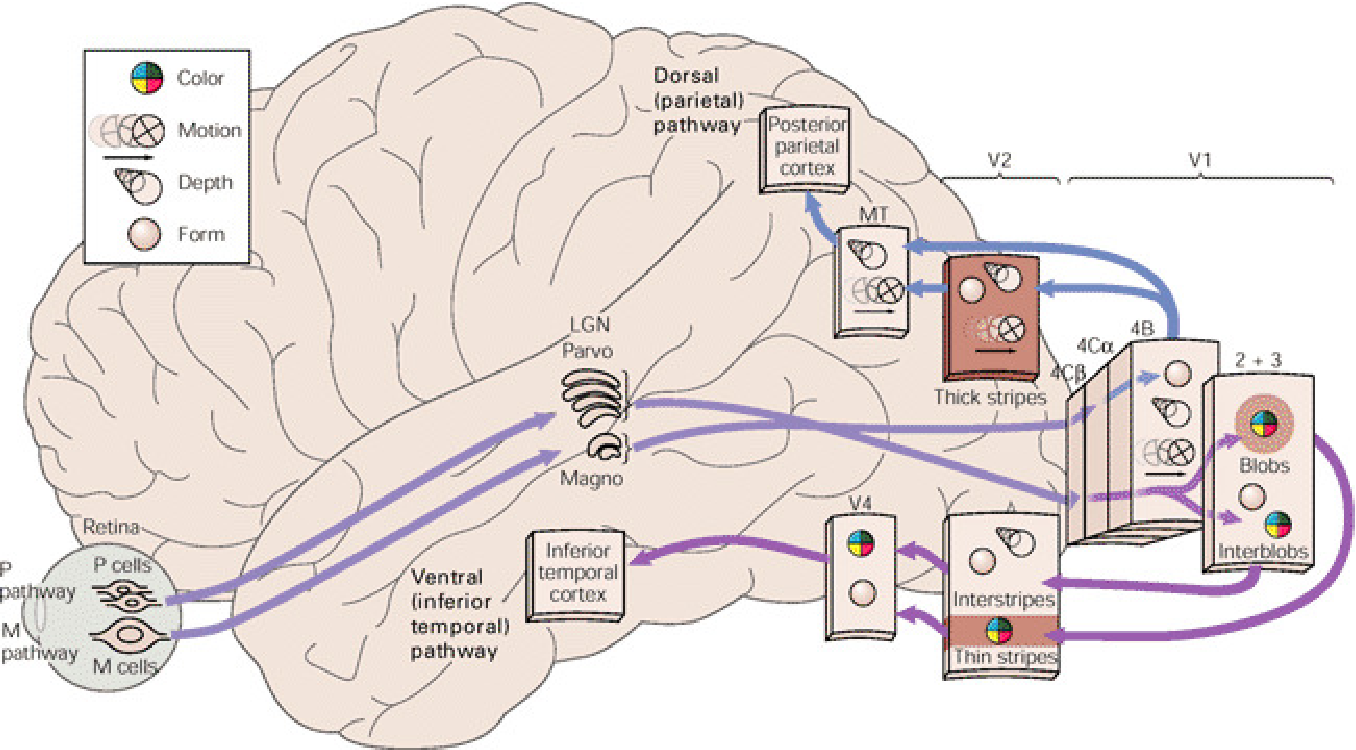
\includegraphics[width=0.9\columnwidth]{visual_pathway.pdf}
         \\
         \raggedleft {\tiny (Van Essen\&Gallant, 1994)}
     \end{minipage}

     \begin{minipage}{0.32\textwidth}
         \centering
         \small
         \textit{Learn} massive data
     \end{minipage}
     \hfill
     \begin{minipage}{0.32\textwidth}
         \centering
         \small
         \textit{simple functions}
     \end{minipage}
     \hfill
     \begin{minipage}{0.32\textwidth}
         \centering
         \small
         \textit{Multi-layered} 
     \end{minipage}

     \vspace{3mm}
    \centering
    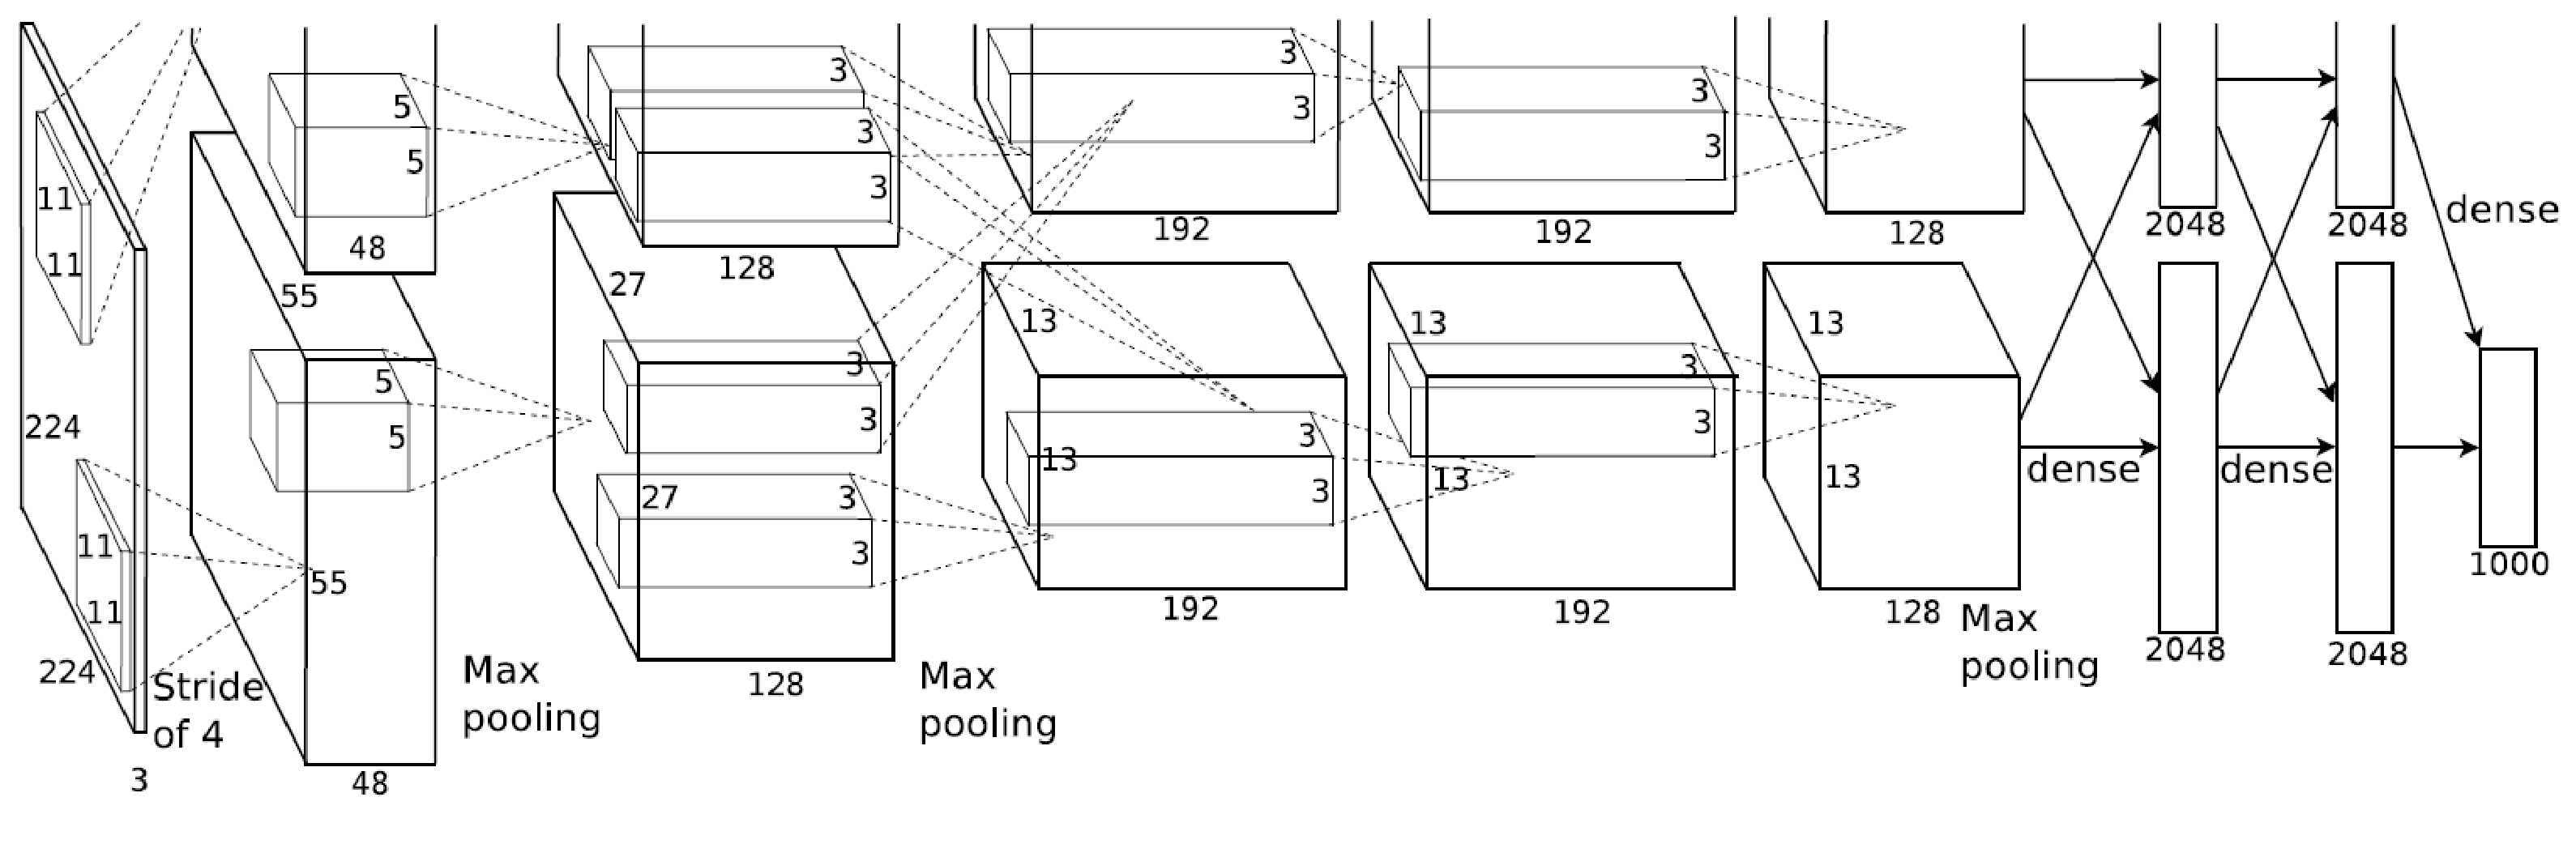
\includegraphics[width=0.8\textwidth]{alex_imagenet}
    \\
    \raggedleft {\scriptsize (Krizhevsky et al., 2012)}

    \vfill

\end{frame}

\begin{frame}
\centering
\emph{Boltzmann machines? I remember working on them in 80s and 90s..}

\vspace{2.5mm}
\begin{flushright}
-- Anonymous Interviewer, 2011 \\ {\small \emph{paraphrased}}
    \end{flushright}
\end{frame}

\begin{frame}{Deep Learning: History}

\begin{enumerate}
\item[1958] Rosenblatt proposed perceptrons 
\item[1982] Hopfield network, SOM {\scriptsize (Kohonen, 1982)}, Neural PCA {\scriptsize (Oja, 1982)}
\item[1985] Boltzmann machines {\scriptsize (Ackley et al., 1985)}
\item[1986] Multilayer perceptrons and backpropagation {\scriptsize (Rumelhart et al., 1986)}
\item[1988] RBF networks {\scriptsize (Broomhead\&Lowe, 1988)}
\item[1989] Autoencoders {\scriptsize (Baldi\&Hornik, 1989)}, Convolutional network {\scriptsize (LeCun, 1989)}
\item[1992] Sigmoid belief network {\scriptsize (Neal, 1992)}
\item[1993] Sparse coding {\scriptsize (Field, 1993)}
\end{enumerate}

\end{frame}

\begin{frame}

\centering
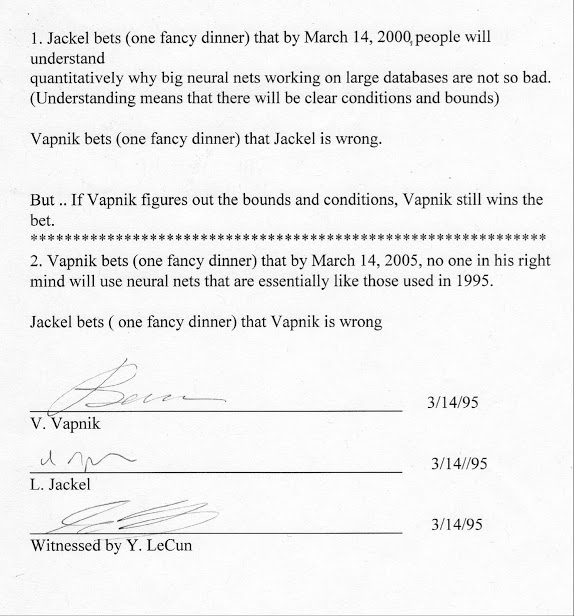
\includegraphics[width=0.80\textwidth]{bet-by-2000.jpg}

\end{frame}

\begin{frame}

\centering
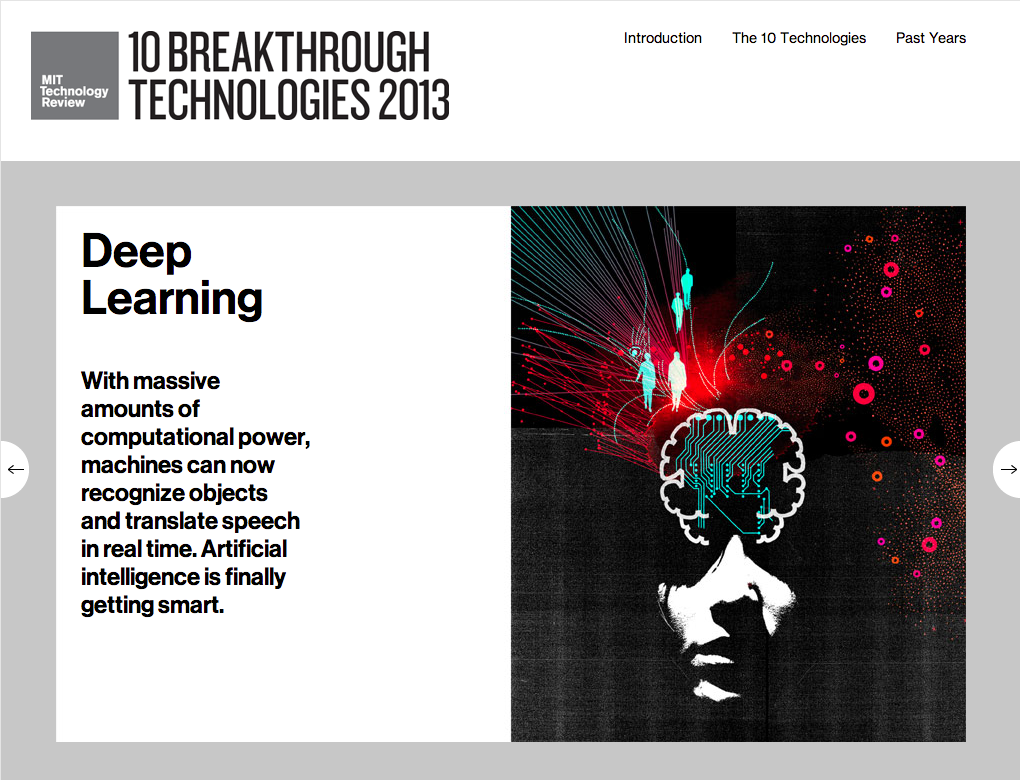
\includegraphics[width=0.85\textwidth]{mit_breakthrough_deepl.png}

%{\small
%\begin{itemize}
%\itemsep 0em
%\item  Object Detection {\scriptsize (Krizhevsky et al., 2012; Ciresan et al., 2012; Goodfellow et al., 2013)} 
%\item Speech Recognition {\scriptsize (Hinton et al., 2012; Dahl et al., 2012; Deng
%        et al., 2013)} 
%\item Natural language processing {\scriptsize (Socher et al., 2011; Mikolov et al., 2010)} 
%\item Transfer learning {\scriptsize (Mesnil et al., 2012)}
%\end{itemize}
%}

\end{frame}

\subsection{What's all this fuss about deep learning?}

\begin{frame}
    \centering 
    Why all this fuss about deep learning now?
\end{frame}

\begin{frame}{ImageNet: ILSVRC 2012 -- Classification Task}

    {\bf Top Rankers}
    {\small
    \begin{enumerate}
        \item {\bf SuperVision: Deep Convolutional Neural Network
            {\scriptsize (Krizhevsky et al.)}}
        \item ISI: SIFT, CSIFT, LBP, GIST + FV + Linear
            classifier {\scriptsize (Gunji et al.)}
        \item OXFORD\_VGG: SIFT + others + FV + SVM
            {\scriptsize (Simonyan et al.)}
        \item XRCE/INRIA: SIFT + others + FV + PQ + SVM
            {\scriptsize (Perronin et al.)}
        \item University of Amsterdam: Color desc. + SVM
            {\scriptsize (van de Sande et al.)}
    \end{enumerate}
    }

    \centering
    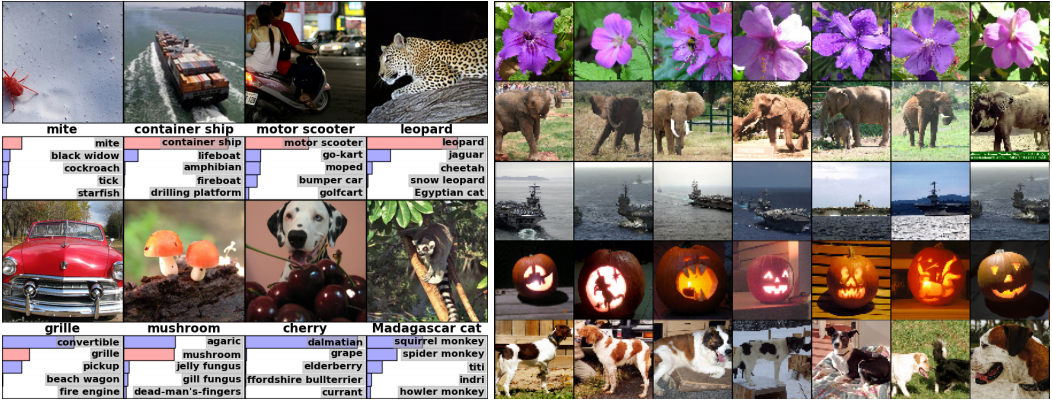
\includegraphics[width=0.8\textwidth]{krizhevsky.png}
    \\
    \raggedleft {\scriptsize (Krizhevsky et al., 2012)}

\end{frame}

\begin{frame}{ImageNet: ILSVRC 2013 -- Classification Task}

    {\small
    \begin{enumerate}
        \item[1] {\bf Clarifi: Deep Convolutional Neural Networks
            {\scriptsize (Zeiler)}}
        \item[\dots] \emph{10+} teams using CNN
        \item[$\circ$] MIL: Local image descriptors + FV + linear
            classifier {\small (Hidaka et al.)}
        \item[\dots] About 3 teams using CNN
        \item[$\circ$] QuantumLeap: 15 features + RVM {\small
            (Shu\&Shu)}
    \end{enumerate}
    }

    \centering
    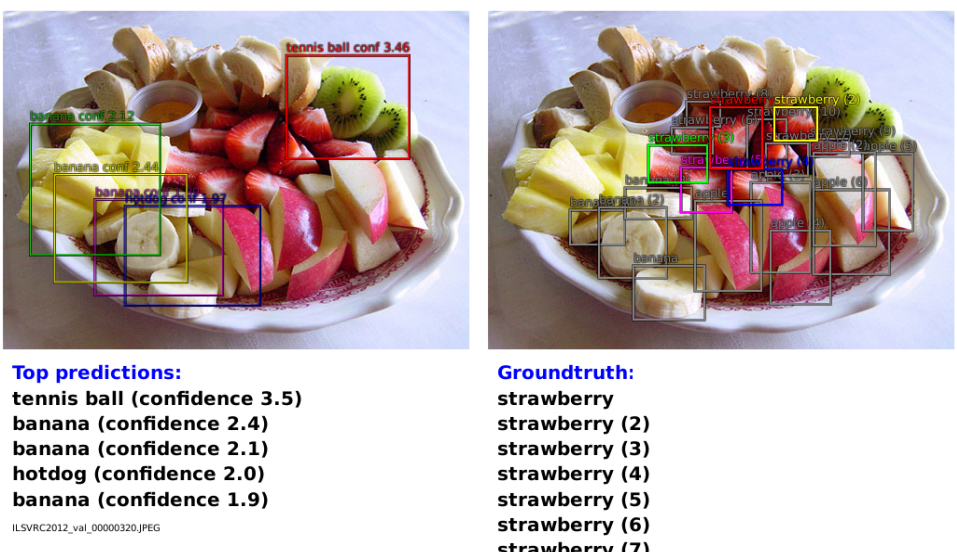
\includegraphics[width=0.75\textwidth]{overfeat.png}

    \vspace{-7mm}
    \raggedleft {\scriptsize (Sermanet et al., 2013)}

\end{frame}

\begin{frame}{You're already using \emph{deep learning}!}

    \begin{minipage}{0.48\textwidth}
        \centering
        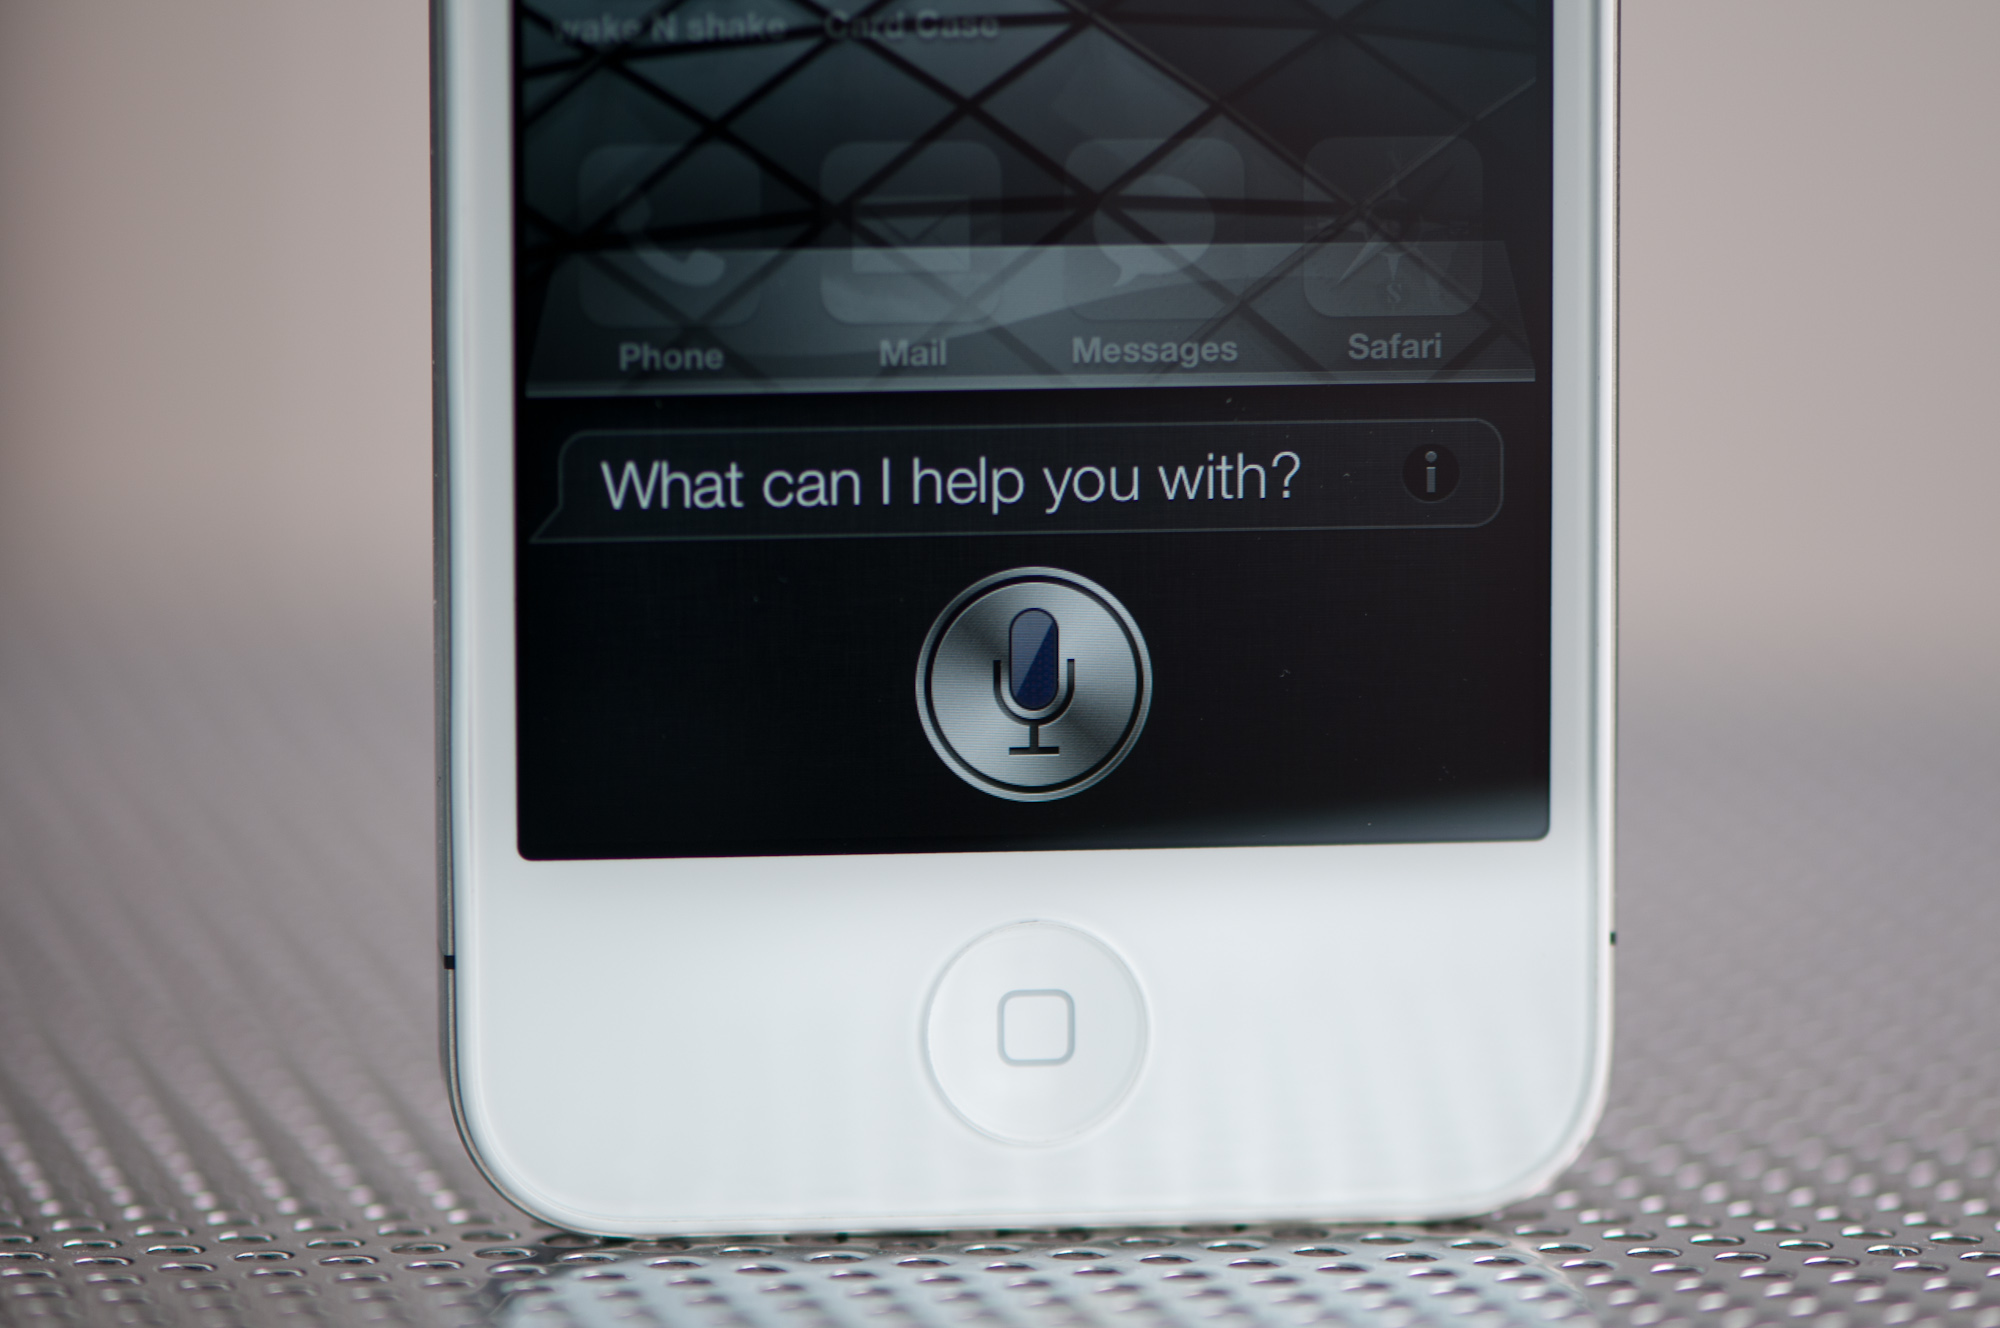
\includegraphics[width=0.9\columnwidth]{siri.jpg}
    \end{minipage}
    \hfill
    \begin{minipage}{0.48\textwidth}
        \centering
        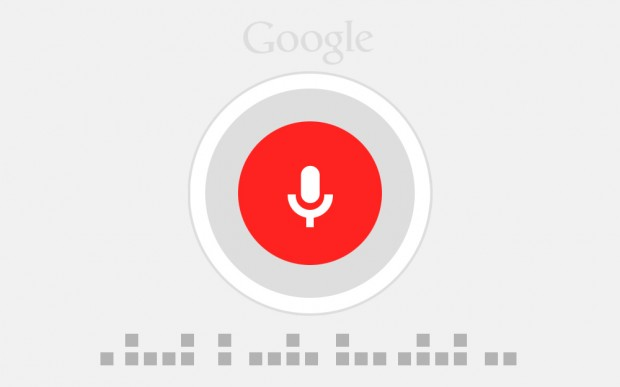
\includegraphics[width=0.9\columnwidth]{googlevoice.jpg}
    \end{minipage}

\end{frame}

\section{Machine Learning vs. Deep Learning}

\begin{frame}
\centering How do you tell deep learning from
\emph{not-so-deep} machine learning?
\end{frame}

\begin{frame}{Not-So-Deep Machine Learning}
    \raggedright
    \begin{enumerate}
        \item Feature engineering $\leftarrow$ {\bf \emph{not learned!}}
        \item \tred{Learning}
        \item \tblue{Inference}
    \end{enumerate}

    \vspace{-24mm}
    \begin{center}
    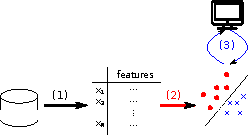
\includegraphics[width=0.8\textwidth]{pipeline1.pdf}
    \end{center}

    \emph{Separation between domain knowledge and general
    machine learning}

\end{frame}

\begin{frame}{Unsupervised Learning of Representation}
    \raggedright
    \begin{enumerate}
    \itemsep 0em
        \item[1a.] Feature engineering
        \item[1b.] Feature/Representation \tred{learning}
        \item[2.] \tred{Learning}
        \item[3.] \tblue{Inference}
    \end{enumerate}

    \vspace{-28mm}
    \begin{center}
    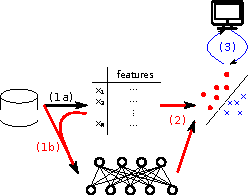
\includegraphics[width=0.8\textwidth]{pipeline2.pdf}
    \end{center}

\end{frame}

\begin{frame}{Deep Learning: toward the \emph{Ultimate} Machine Learning?}
    \raggedright
    \begin{enumerate}
        \item Jointly \tred{learn} \emph{everything}
        \item \tblue{Inference}
    \end{enumerate}

    \vspace{-24mm}
    \begin{center}
    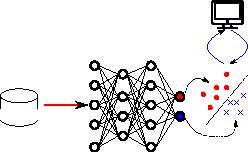
\includegraphics[width=0.8\textwidth]{pipeline3.pdf}
    \end{center}

    \raggedleft
    \emph{The data decides}
    {\small --Yoshua Bengio}

\end{frame}

\section{Why deep learning?}


\subsection{Why now? And what happens next?}

\begin{frame}
    \centering
Why now? Why not 20 years ago?

\end{frame}

\begin{frame}{What has happened in last 20+ years?}
    \begin{itemize}
        \item We have connected the dots, e.g.,
            \begin{itemize}
                \item PCA $\Leftrightarrow$ Neural PCA
                    $\Leftrightarrow$
                    Probabilistic PCA $\Leftrightarrow$ 
                    Autoencoder
                \item Autoencoder $\Leftrightarrow$ Belief
                    network $\Leftrightarrow$ Restricted
                    Boltzmann machine
            \end{itemize}
        \item We understand \tred{learning} better
            \begin{itemize}
                \item Learning \emph{is} but \emph{is not} optimization 
                \item No need to be scared of non-convex
                    optimization
            \end{itemize}
        \item We understand better how \tred{learning} and
            \tblue{inference} are intermingled
        \item \textcolor{gray}{The exponential growth of the amount of data
            and the computational power}
    \end{itemize}
\end{frame}


\begin{frame}[fragile,plain]{And Beyond..}

    \hspace*{-10.5mm}
    \includegraphics[width=\paperwidth]{ian1.png}

    \raggedleft {\scriptsize (Goodfellow, 2013)}
    
\end{frame}



%%%%%%%%%%%%%%%%%%%%%%%%%%%%%%%%%%%%%%%%%%%%%%%%%%%%%%%%%%%%%%%%%%%%%%%%%%%%%%%%%%%%%%%%%%%%%%
%\begin{frame}{Is Learning Optimization?}

%    \centering
%    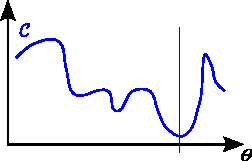
\includegraphics[width=0.5\textwidth]{cost_true.pdf}

%    \begin{minipage}{0.48\textwidth}
%        \textbf{\emph{Yes}}
%    \end{minipage}
%    \hfill
%    \begin{minipage}{0.48\textwidth}
%    %\emph{No}
%    \end{minipage}

%    %\vspace{1mm}

%    \begin{minipage}[t]{0.48\textwidth}
%        \vspace{0pt}
%    Learning minimizes a cost function $\color{blue}{\CC}$ with respect to
%    $\MM$ given a data distribution $p_D$

%    \end{minipage}
%    \hfill
%    \begin{minipage}[t]{0.48\textwidth}
%    %    \vspace{0pt}
%    %$\color{blue}{\CC}$ is \emph{not} available, but $\color{red}{\tilde{\CC}}$ based
%    %on the samples from $p_D$.

%    \end{minipage}

%\end{frame}

%\begin{frame}{Is Learning Optimization?}

%    \centering
%    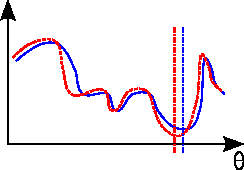
\includegraphics[width=0.5\textwidth]{cost_both.pdf}

%    \begin{minipage}{0.48\textwidth}
%        \textbf{\emph{Yes}}
%    \end{minipage}
%    \hfill
%    \begin{minipage}{0.48\textwidth}
%        \textbf{\emph{No}}
%    \end{minipage}

%    %\vspace{1mm}

%    \begin{minipage}[t]{0.48\textwidth}
%        \vspace{0pt}
%    Learning minimizes a cost function $\color{blue}{\CC}$ with respect to
%    $\MM$ given a data distribution $p_D$

%    \end{minipage}
%    \hfill
%    \begin{minipage}[t]{0.48\textwidth}
%        \vspace{0pt}
%    $\color{blue}{\CC}$ is \emph{not} available, but $\color{red}{\tilde{\CC}}$ based
%    on the samples from $p_D$.

%    \end{minipage}

%\end{frame}

\end{document}
